{For each of the given points give two sets of polar coordinates that identify it, where $-\pi\leq \theta\leq \pi$.

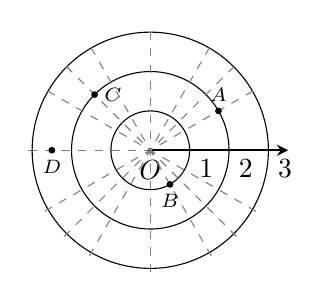
\begin{tikzpicture}[scale=.5]
	\draw [dashed,gray] (-3.1,0) -- (0,0);
	\draw[thick,->,>=stealth] (0,0) node [below] {$O$} -- (3.5,0) ;
	\filldraw (0,0) circle (1.5pt);
	\foreach \x in {1,2,3}
	{\draw (0,0) circle (\x cm);
	\draw (\x,0) node [below right] {\x};
	}
	\foreach \x in {30,45,60,90,120,135,150}
	{\draw [rotate=\x,dashed,gray] (-3.1,0) -- (3.1,0);
	}
	\filldraw (xyz polar cs: angle=30,radius=2) circle (2pt) node [above] {\scriptsize $A$}
	      (xyz polar cs: angle=-60,radius=1)circle (2pt) node [below] {\scriptsize $B$}
				(xyz polar cs: angle=135,radius=2)circle (2pt) node [right] {\scriptsize $C$}
				(xyz polar cs: angle=180,radius=2.5)circle (2pt) node [below] {\scriptsize $D$};
	
\end{tikzpicture}	
}
{$A=P(2,\pi/6)$ and $P(-2,-5\pi/6)$;

$B=P(1,-\pi/3)$ and $P(-1,2\pi/3)$;

$C=P(2,3\pi/4)$ and $P(-2,-\pi/4)$;

$D=P(2.5,\pi)$ and $P(2.5,-\pi)$;

	}
